% Copyright 2004 by Till Tantau <tantau@users.sourceforge.net>.
%
% In principle, this file can be redistributed and/or modified under
% the terms of the GNU Public License, version 2.
%
% However, this file is supposed to be a template to be modified
% for your own needs. For this reason, if you use this file as a
% template and not specifically distribute it as part of a another
% package/program, I grant the extra permission to freely copy and
% modify this file as you see fit and even to delete this copyright
% notice. 

%Use this to print without animation
\documentclass[handout, xcolor={dvipsnames}]{beamer}

%Use this to print WITH animation
%\documentclass[xcolor={dvipsnames}]{beamer}

% There are many different themes available for Beamer. A comprehensive
% list with examples is given here:
% http://deic.uab.es/~iblanes/beamer_gallery/index_by_theme.html
% You can uncomment the themes below if you would like to use a different
% one:
%\usetheme{AnnArbor}
%\usetheme{Antibes}
%\usetheme{Bergen}
\usetheme{Berkeley}
%\usetheme{Berlin}
%\usetheme{Boadilla}
%\usetheme{boxes}
%\usetheme{CambridgeUS}
%\usetheme{Copenhagen}
%\usetheme{Darmstadt}
%\usetheme{default}
%\usetheme{Frankfurt}
%\usetheme{Goettingen}
%\usetheme{Hannover}
%\usetheme{Ilmenau}
%\usetheme{JuanLesPins}
%\usetheme{Luebeck}
%usetheme{Madrid}
%\usetheme{Malmoe}
%\usetheme{Marburg}
%\usetheme{Montpellier}
%\usetheme{PaloAlto}
%\usetheme{Pittsburgh}
%\usetheme{Rochester}
%\usetheme{Singapore}
%\usetheme{Szeged}
%\usetheme{Warsaw}
\usepackage{cancel}
\usepackage{amsmath,amsthm,verbatim,amssymb,amsfonts,amscd, graphicx, amsmath}
\usepackage{soul} %for line through a text
\usepackage{graphics}
\usepackage{mathrsfs} %mathscr font
\usepackage{fourier} %doublestruck
\usepackage{nccmath} %aligning equatinos as required
\usepackage{tikz} %drawing
\usetikzlibrary{backgrounds} %figure -- useful for framing
\usepackage{caption} %add caption to figure
\usepackage{float} %stopf "figure" from floating
\usepackage{pgfplots} %graphs
\pgfplotsset{my style/.append style={axis x line=middle, axis y line= middle, xlabel={$v_k$}, ylabel={$y_k$}}}
\pgfplotsset{my style2/.append style={axis x line=middle, axis y line= middle, xlabel={$v$}, ylabel={$y$}}}
%%to fix quotes
\usepackage [autostyle, english = british]{csquotes}
\MakeOuterQuote{"}
%%

%\usepackage[dvipsnames]{xcolor}

%%Bibliography
\usepackage[
    %backend=biber, 
    natbib=true,
    style=numeric,
    sorting=none
]{biblatex}
\addbibresource{cite.bib}
%%


%%


%for ayer separation space in ANN drawings
\def\layersepshort{2.5cm}
\def\layersepVshort{2.0cm}
\def\layersep{3.5cm}

%%%%%%%%%%%%%%%%%%%%%%%%%%%%%%%%%%%%%%%%%%%%%%%%%%%%%%

\title{MLSQL: Machine Learning Meets SQL}

% A subtitle is optional and this may be deleted
\subtitle{}

\author{V. Chakraborty and G. Muktadir
%\inst{1}
}
% - Give the names in the same order as the appear in the paper.
% - Use the \inst{?} command only if the authors have different
%   affiliation.

\institute[Uni. of California] % (optional, but mostly needed)
{
  \inst{}%
  \textit{CMPS 203, Spring 2019}\\
 }
% - Use the \inst command only if there are several affiliations.
% - Keep it simple, no one is interested in your street address.

\date{30 May, 2019}
% - Either use conference name or its abbreviation.
% - Not really informative to the audience, more for people (including
%   yourself) who are reading the slides online

\subject{CMPS 203 Course Project}
% This is only inserted into the PDF information catalog. Can be left
% out. 

% If you have a file called "university-logo-filename.xxx", where xxx
% is a graphic format that can be processed by latex or pdflatex,
% resp., then you can add a logo as follows:

\pgfdeclareimage[height=1.5cm]{university-logo}{uc_logo.png}
\logo{\pgfuseimage{university-logo}}

% Delete this, if you do not want the table of contents to pop up at
% the beginning of each subsection:
\AtBeginSubsection[]
{
  \begin{frame}<beamer>{Outline}
    \tableofcontents[currentsection,currentsubsection]
  \end{frame}
}

% Let's get started
\begin{document}

\begin{frame}
  \titlepage
\end{frame}

\begin{frame}{Outline}
  \tableofcontents
  % You might wish to add the option [pausesections]
\end{frame}

% Section and subsections will appear in the presentation overview
% and table of contents.
\section{Introduction}
\begin{frame}{Motivation}{}
  \begin{itemize}
  \item<1-> {
   Objective
   \begin{itemize}
       \item<1->  A vast amount of data around us these days (the usual Big Data spiel!)
       \vspace{.2in}
       \item<2-> Machine Learning, a lot like the President's impeachment
        \begin{itemize}
            \item<3-> Everyone is excited about it 
            \item<4-> Everyone is talking about it
            \item<5-> No one (very few) is really doing it!
        \end{itemize}
        \vspace{.2in}
       \item<6-> Popularity of SQL - extremely commonplace
       \begin{figure}
           \centering
           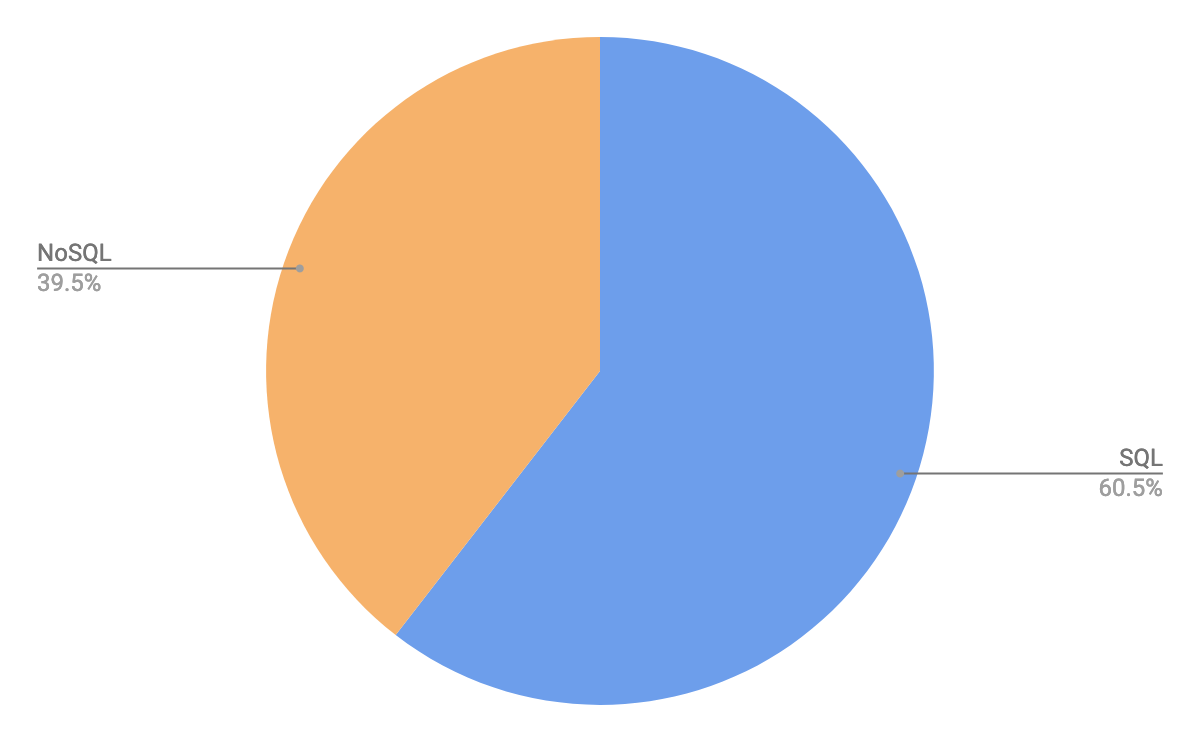
\includegraphics[scale = 0.1]{SQL_no.png}
           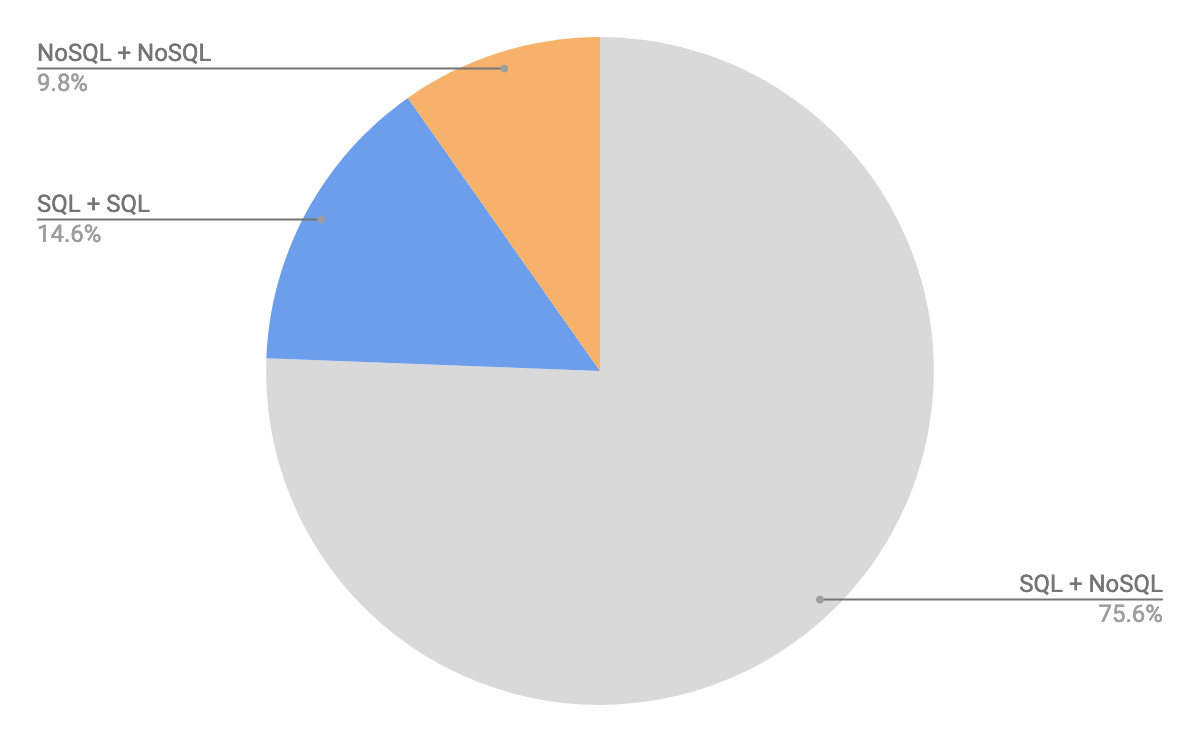
\includegraphics[scale = 0.1]{SQL_usage.png}
           \caption{Prevalence of SQL Databses}
           \label{fig:sql_prev}
       \end{figure}
   \end{itemize}
  }

  \end{itemize}
\end{frame}

\begin{frame}{Motivation}{}
  \begin{itemize}
  \item<1-> {
   Subjective
   \begin{itemize}
       \item<1->  Python - extremely popular, host of libraries
       \vspace{.2in}
       \item<2-> SQLite
        \begin{itemize}
            \item<3-> Portability 
            \item<4-> Throughput
            \item<5-> Popularity
        \end{itemize}
        \vspace{.2in}
       \item<6-> Popularity of SQL - extremely commonplace
       \begin{figure}
           \centering
           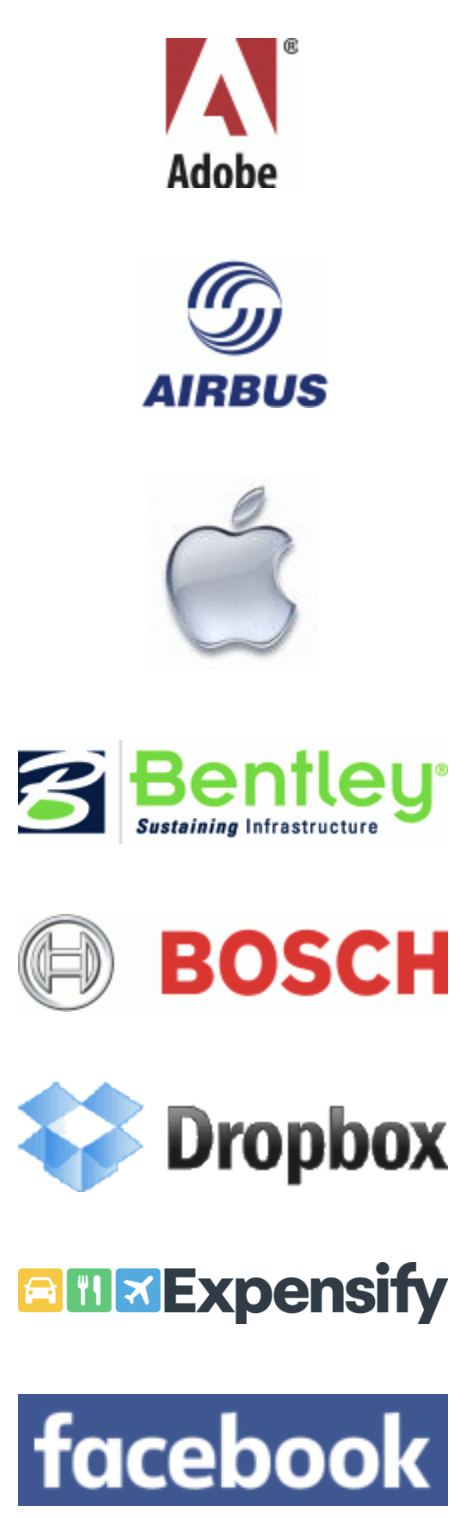
\includegraphics[scale = 0.1]{SQL_use.png}
           \caption{SQLite usage in industry}
           \label{fig:sql_prev}
       \end{figure}
   \end{itemize}
  }

  \end{itemize}
\end{frame}

\begin{frame}{Motivation}{}
  \begin{itemize}
  \item<1-> {
   What we found helpful?
   \begin{itemize}
       \item<1->  Theoretical foundation of Relation DB model -- long tested and still popular
       \vspace{.2in}
       \item<2-> Experience with 
        \begin{itemize}
            
            \item<3-> Tenserflow 
            \item<4-> Scikit Learn
            \item<5-> SQL and no SQL databases
            \item<6-> Pytorch
            \item<7-> Theano
            \item<8-> Data Analysis
            \item<9-> Machine Learning
        \end{itemize}
        \vspace{.2in}
       \item<10-> Distributed Systems
   \end{itemize}
  }

  \end{itemize}
\end{frame}
\section{MLSQL}
%%%
\begin{frame}{Overview}{}
  \begin{figure}
      \centering
      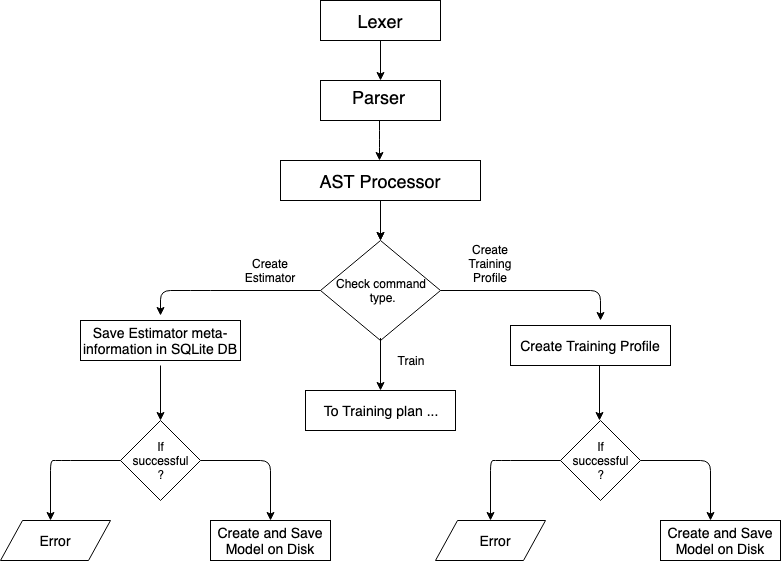
\includegraphics[scale = 0.45]{flow_chart_broad.png}
      \caption{MLSQL}
      \label{fig:flow_broad}
  \end{figure}
\end{frame}

\begin{frame}{Overview}{Training}
  \begin{figure}
      \centering
      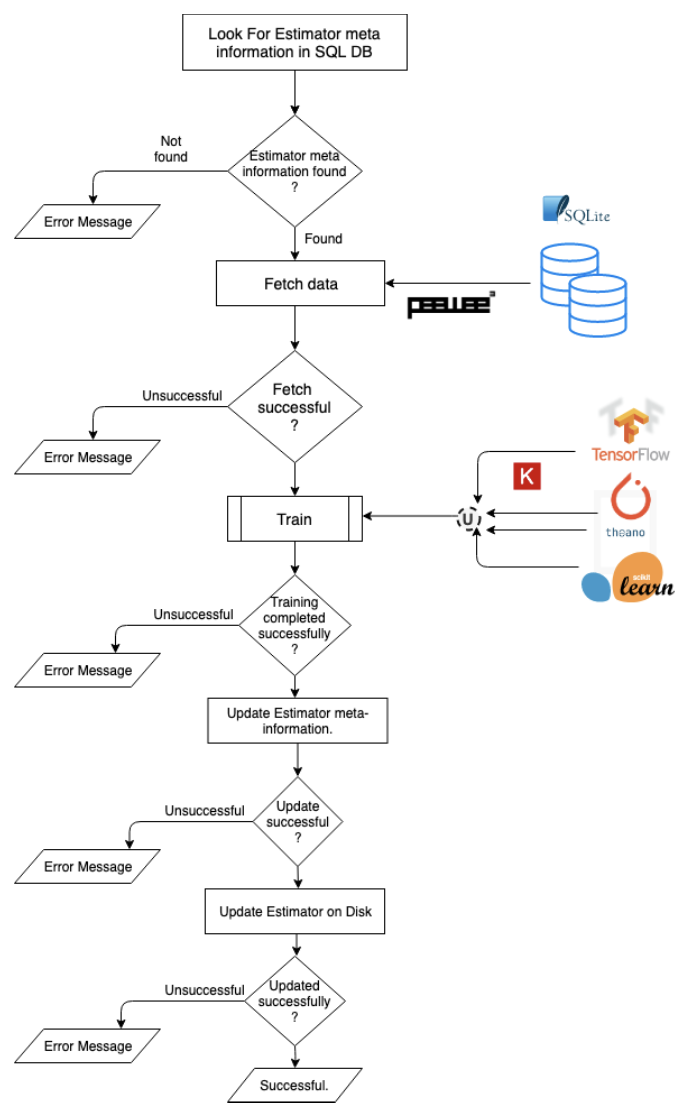
\includegraphics[scale = 0.35]{SQL_train.png}
      \caption{Flow to train in MLSQL}
      \label{fig:flow_train}
  \end{figure}
\end{frame}

\section{Syntax}
\begin{frame}{Example}{Linear Regression}
  \begin{itemize}
  \item<1-> {
   \textbf{Create a model}
   \\
  }
  \texttt{CREATE ESTIMATOR \textcolor{blue}{salaryPred} \\ TYPE \textcolor{Gray}{LR} FORMULA
  \textcolor{Gray}{\$salary$\sim$years$\sim$...\$} }
  \begin{itemize}
      \item attributes in \texttt{FORMULA} must be names of columns in tables of the dataset that will be used.
  \end{itemize}
  \vspace{.1in}
  \item<2->{
  \textbf{Create a training profile}
  \\
  \texttt{CREATE TRAINING PROFILE \textcolor{red}{salaryProfile} \\ 
  WITH [ SELECT \textcolor{Gray}{*} FROM \textcolor{brown}{salary}];}
  }
  \vspace{.1in}
  \item<3->{
  \textbf{Select the database}
  \\
  \texttt{USE \textcolor{Gray}{'data/salarydb.db';}}
  }  
  \vspace{.1in}
  \item<4->{
 \textbf{ Training an estimator with a training profile}
  \\
  \textt{
  TRAIN \textcolor{blue}{salaryPred} WITH TRAINING PROFILE \textcolor{red}{salaryProfile};
  }
  
  }
  \end{itemize}
\end{frame}

\begin{frame}{Syntax}{"Grammar Rule"}
  \begin{itemize}
  \item<1-> {Estimator
     \begin{figure}
         \centering
         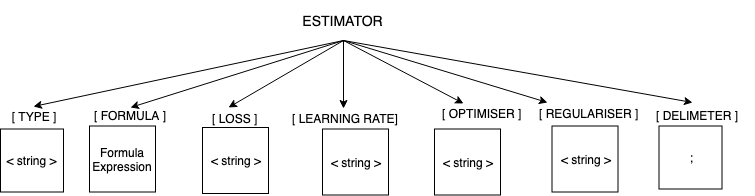
\includegraphics[scale = 0.25]{EstimatorTree.png}
         \caption{Estimator Attributes}
         \label{fig:Est_tree}
     \end{figure}
  }
  \item<2->{Training Profile
       \begin{figure}
         \centering
         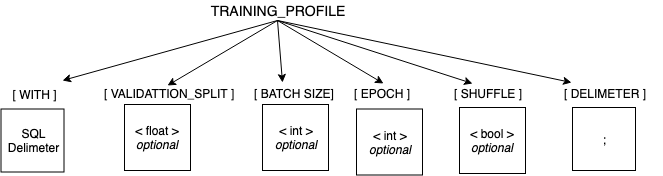
\includegraphics[scale = 0.25]{TrainProfile_Tree.png}
         \caption{Training Profile Attributes}
         \label{fig:Est_tree}
     \end{figure}
  
  }
     
  \end{itemize}
\end{frame}

\begin{frame}{So what's happening?}
\begin{figure}
    \centering
    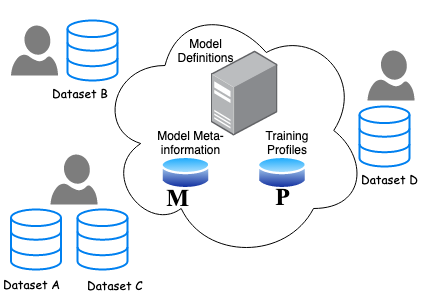
\includegraphics[scale = 0.35]{System_diag.png}
    \caption{MLSQL - Overview}
    \label{fig:system_overview}
\end{figure}
\begin{itemize}
    \item Create model. Store meta-information in database $M$ and the actual model to disk.
    \item Create training profile. Store profile in database $P$.
    \item Use a model from $M$ with profile from $P$ on a dataset of the client's choice.
\end{itemize}
    
\end{frame}
%%%%%%

\section{Design Choices}

\begin{frame}{A Specific Design Choice}{Where to place the model/estimator?}
  \begin{itemize}
      \item<1-> Two alternatives
      \vspace{.2in}
      \begin{itemize}
          \item<2-> Place the model \textcolor{blue}{inside} the database
          \begin{itemize}
              \item<3-> Better portability
          \end{itemize}
          \vspace{.2in}
          \item<4-> Place it \textcolor{blue}{outside} the database
          \begin{itemize}
              \item<5-> Better reusability
              \item<6-> Use the same model on different datasets/databases
              \item<7-> Share the same model
              \item<8-> Replicate model for production
          \end{itemize}
      \end{itemize}
      \vspace{.2in}
      \item<9-> We place it \textcolor{blue}{outside} the database
      \begin{itemize}
          \item<10-> We foresee a setting in which MLSQL is used to create a model and used with different data-sets.
          \item<11-> Trade \textcolor{red}{portability} for \textcolor{ForestGreen}{reusability}
          \item<12-> \textit{Training Profile can be created by a domain expert. But the dataset can be changed by someone who is not.}
      \end{itemize}
  \end{itemize}
  
  
\end{frame}
\begin{frame}{Other Design Choices}{}
  \begin{itemize}
   \item Why SQL?
    \begin{itemize}
        \item<1-> Recent progress -- Tensor Flow API for javascript users
        \item<2-> We are providing ML to SQL users
        \item<3-> Next... \cancelto{\textcolor{red}{ALL}}{\text{ ML for HTML and \LaTeX users !!} }
    \end{itemize}
    \vspace{.2in}
   \item SQLite3 and Pewee ORM
   \begin{itemize}
       \item "virtual object database" that can be used from within the programming language
   \end{itemize}
  \end{itemize}
\end{frame}
%%%

\section{Novelty}
\begin{frame}{Is this idea completely new?}{Novelty}
  \begin{itemize}
  \item<1-> {
   Surely not! However, ours is pretty dope
   \begin{itemize}
       \color{ForestGreen}
       \item opensource
       \item No "new" language
       \item Abstracts using ML into two steps
        \begin{itemize}
        \color{blue}
            \item Model Engineering (for trained experts)
            \item Model Implementation (for everyone)
        \end{itemize}
       \item Try to minimise "shoot-in-the-dark" trend of machine learning.
   \end{itemize} 
  }
  \vspace{.2in}
  \item<2->{
  Here are some tools that inspired us...
  }
      \begin{itemize}
          \item<3-> Uber's \textcolor{red}{Queryparser} \cite{QueryParser} 
          \begin{itemize}
              \item<3-> no ML but helped us conceive the design of our parser
          \end{itemize}
          
          \vspace{.2in}
          
          \item<4-> Google's \textcolor{red}{BigQuery} \cite{BigQuery} used in conjunction with MapReduce
          \begin{itemize}
          \item<4-> serverless service
          \item<4-> complicated code
          \item<4-> expensive
          \end{itemize}
          
      \end{itemize}
  \end{itemize}
\end{frame}


\begin{frame}{Novelty}{Continued...}
    \begin{itemize}
        \item<1-> Microsoft's \textcolor{red}{SQL Server 2017} \cite{SQLserver}
          \begin{itemize}
              \item<1-> separate core language which is quite different from other DB applications
              \item<1-> expensive
              \item<1-> companies that want to upgrade need to teach current employees how to work with the application
              \item<1-> .NET framework dependent 
          \end{itemize}
    \end{itemize}
\end{frame}
%%%

%****


%%%%%%%%%%%%%%%%%%%%%%%%%%%%%%%%%%
% Placing a * after \section means it will not show in the
% outline or table of contents.
%\section*{Summary}

%\begin{frame}{Summary}
  %\begin{itemize}
  %\item
   % The \alert{first main message} of your talk in one or two lines.
  %\item
    %The \alert{second main message} of your talk in one or two lines.
  %\item
    %Perhaps a \alert{third message}, but not more than that.
  %\end{itemize}
  
  %\begin{itemize}
  %\item
    %Outlook
    %\begin{itemize}
    %\item
      %Something you haven't solved.
    %\item
      %Something else you haven't solved.
    %\end{itemize}
  %\end{itemize}
%\end{frame}



% All of the following is optional and typically not needed. 
\appendix
\section<presentation>*{\appendixname}
\subsection<presentation>*{Bibliography}

\begin{frame}[allowframebreaks]
  \frametitle<presentation>{Bibliography}
    
  \printbibliography
  \centering
    Thank you!
\end{frame}

\end{document}



